\documentclass[11pt,a4paper]{article}
\usepackage[margin=1in]{geometry}
\usepackage{graphicx}
\title{Client Dominance and Agent Co-evaluation in ERC8004\\Science-Chief Report}
\author{Science-Chief}
\date{2026-03-08}
\begin{document}
\maketitle

\section*{Introduction}
A critical risk in reputation systems is evaluator dominance: if a very small subset of clients produces most feedback, the reputation layer can become structurally biased and fragile. This report quantifies client-side concentration and formalizes the agent co-evaluation matrix at the core of projection-based network analysis.

\section*{Data and Setup}
We use ERC8004 Ethereum feedback events from \texttt{reputation\_newfeedback.csv}. Each event links a client address to an agent identifier. From this event table, we construct three objects: (i) feedback count per client, (ii) number of distinct agents rated per client, and (iii) co-evaluation matrix among agents.

\section*{Methods}
Let $k_c$ be the number of feedback events emitted by client $c$. We study the empirical distribution of $k_c$ and concentration metrics (Lorenz/Gini/HHI/top-share).

For agent co-evaluation, define the matrix
\[
M_{ij} = \#\{c: c\ \mathrm{rates}\ i\ \mathrm{and}\ j\}.
\]
This matrix is the structural core of agent projection: large $M_{ij}$ implies strong evaluator-overlap between agents $i$ and $j$.

\section*{Results}
The concentration metrics are extreme. Out of 568 active clients and 2,776 total feedback events, the top 1\% of clients emits about 70.3\% of all feedback, and the top 10 clients emit about 71.9\%. The estimated Gini coefficient is 0.7808 and the HHI is 0.2219, both indicating very high concentration. The ratio between maximum and median client activity is 1215, which confirms a strongly skewed evaluator distribution.

Figure 1 (histogram) and Figure 2 (CCDF) show a heavy-tailed activity pattern: many low-activity clients coexist with a very small high-activity tail. Figure 3 (Lorenz) visualizes the same dominance in cumulative form.

The co-evaluation matrix is computed in long format and summarized visually for top agents (Figure 4). This confirms that projection edges are not random artifacts; they are induced by overlapping evaluator sets. Hence, projection analysis is meaningful, but it inherits concentration bias from the evaluator layer.

\begin{figure}[htbp]
\centering
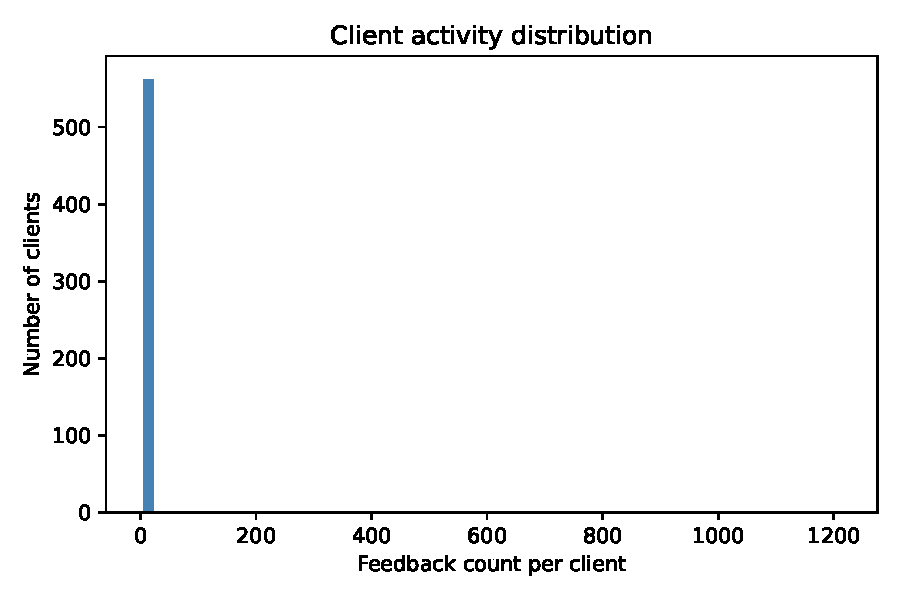
\includegraphics[width=0.82\textwidth]{figures/client_feedback_count_hist.pdf}
\caption{Distribution of feedback events per client.}
\end{figure}

\begin{figure}[htbp]
\centering
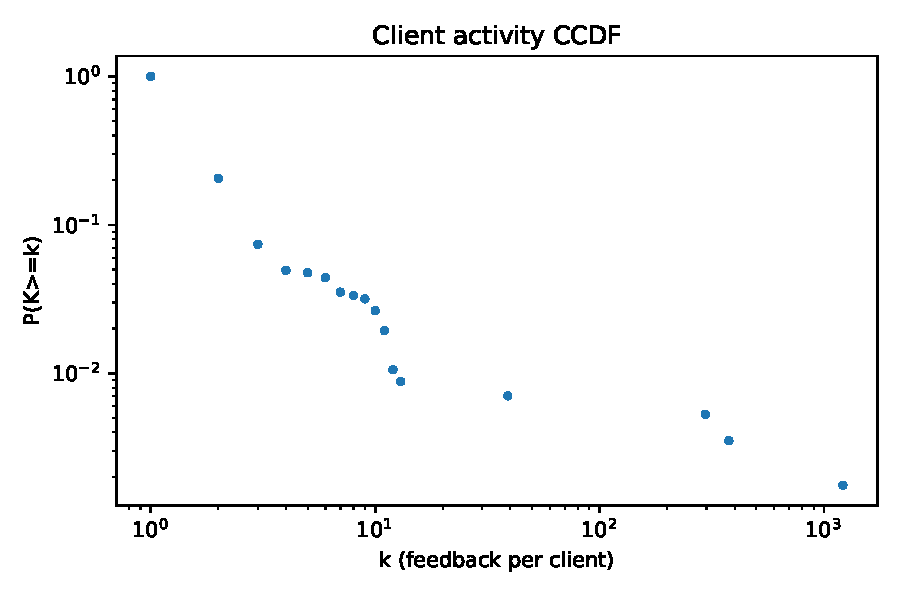
\includegraphics[width=0.82\textwidth]{figures/client_feedback_count_ccdf.pdf}
\caption{CCDF of client activity (log-log view).}
\end{figure}

\begin{figure}[htbp]
\centering
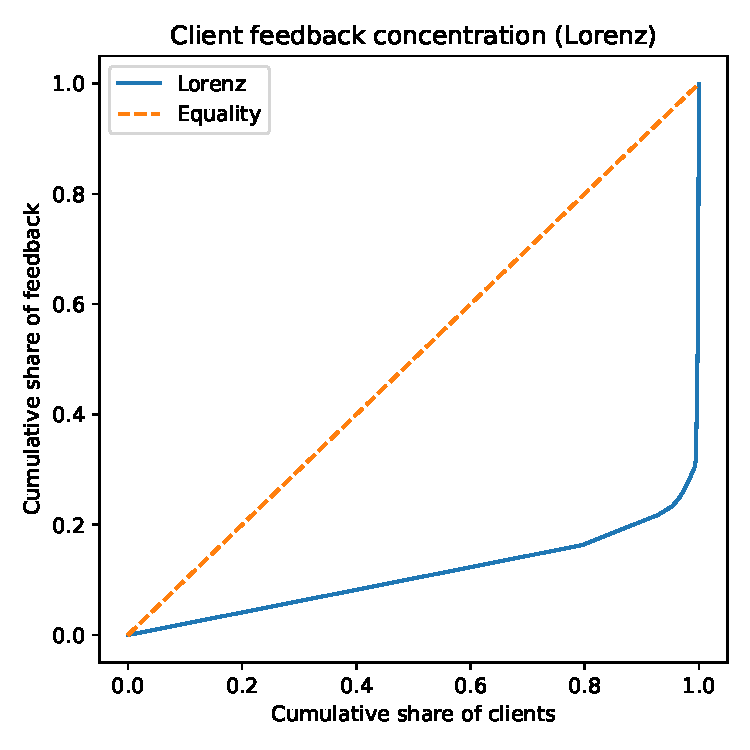
\includegraphics[width=0.75\textwidth]{figures/client_lorenz_curve.pdf}
\caption{Lorenz curve for client-side feedback concentration.}
\end{figure}

\begin{figure}[htbp]
\centering
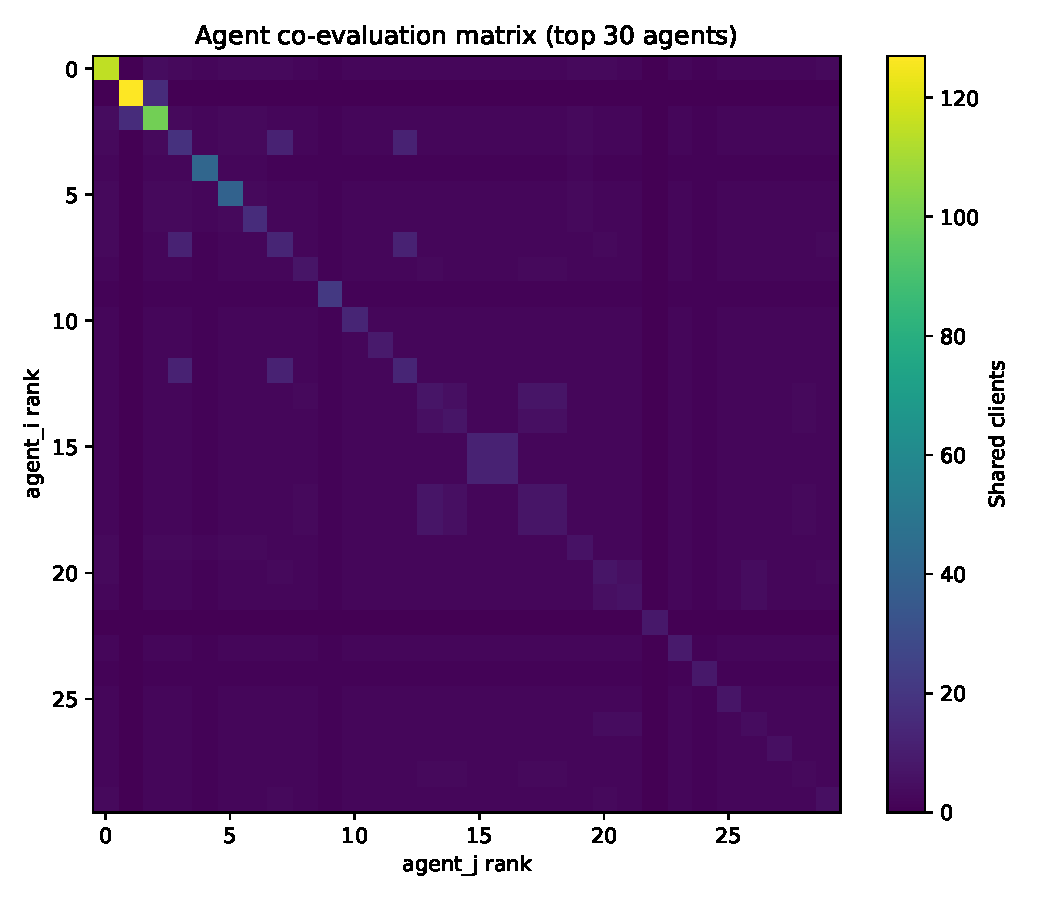
\includegraphics[width=0.82\textwidth]{figures/agent_coevaluation_heatmap_top30.pdf}
\caption{Agent co-evaluation matrix heatmap (top 30 agents by activity).}
\end{figure}

\section*{Interpretation}
Scientifically, this is a strong dominance signal: feedback issuance is highly centralized. Therefore, any reputation interpretation that assumes broad, independent evaluator participation is currently invalid. The agent projection remains informative, but should be interpreted with explicit dominance caveats and robustness checks (e.g., de-biasing by high-activity clients).

\section*{Conclusion}
The analysis answers the core question clearly: yes, a very small subset of clients contributes the majority of feedback and can dominate the reputation layer. The co-evaluation matrix $M_{ij}$ is correctly constructed and confirms the structural basis of agent projection, but the projection must be interpreted under concentration-aware controls.

\section*{Appendix: Source Paths}
\textbf{Figures}\\
\begin{itemize}
\item \texttt{workspaces/science-chief/outbox/Reports/CLIENT\_DOMINANCE\_COEVAL\_2026-03-08/figures/client\_feedback\_count\_hist.pdf}
\item \texttt{workspaces/science-chief/outbox/Reports/CLIENT\_DOMINANCE\_COEVAL\_2026-03-08/figures/client\_feedback\_count\_ccdf.pdf}
\item \texttt{workspaces/science-chief/outbox/Reports/CLIENT\_DOMINANCE\_COEVAL\_2026-03-08/figures/client\_lorenz\_curve.pdf}
\item \texttt{workspaces/science-chief/outbox/Reports/CLIENT\_DOMINANCE\_COEVAL\_2026-03-08/figures/agent\_coevaluation\_heatmap\_top30.pdf}
\end{itemize}

\textbf{Tables}\\
\begin{itemize}
\item \texttt{workspaces/science-chief/outbox/Reports/CLIENT\_DOMINANCE\_COEVAL\_2026-03-08/tables/client\_feedback\_counts.csv}
\item \texttt{workspaces/science-chief/outbox/Reports/CLIENT\_DOMINANCE\_COEVAL\_2026-03-08/tables/agents\_per\_client.csv}
\item \texttt{workspaces/science-chief/outbox/Reports/CLIENT\_DOMINANCE\_COEVAL\_2026-03-08/tables/client\_concentration\_summary.csv}
\item \texttt{workspaces/science-chief/outbox/Reports/CLIENT\_DOMINANCE\_COEVAL\_2026-03-08/tables/agent\_coevaluation\_matrix\_long.csv}
\item \texttt{workspaces/science-chief/outbox/Reports/CLIENT\_DOMINANCE\_COEVAL\_2026-03-08/tables/agent\_coevaluation\_top50\_pairs.csv}
\end{itemize}

\end{document}
